\chapter{Scripts And Tools}






\section{Create Effect Combinations}
\subsection{Overview}
The \texttt{create\_effect\_combinations.py} script is a Python 3 tool designed to generate all possible combinations of a sentence or set of sentences by replacing placeholders with values defined in external text files. It is ideal for creating permutations of text templates, such as game effects, test cases, or parameterized strings, where placeholders (e.g., \texttt{<rank>}) represent variable elements. The tool supports nested placeholders, numeric offsets (e.g., \texttt{<rank+1>}), and configurable post-processing to clean, filter, and refine the output.

This script automates the generation of exhaustive text combinations, with output that can be written to a file or displayed in the terminal. Configuration files enhance flexibility by allowing users to customize filtering and phrase replacements without modifying the source code.

\subsection{Purpose}
The \texttt{create\_effect\_combinations.py} script aims to streamline the creation of text variations from templates. Common use cases include:
\begin{itemize}
    \item Generating card or spell effects for games (e.g., "Draw \texttt{<number>} cards").
    \item Producing test data for software validation.
    \item Creating parameterized strings for simulations or documentation.
\end{itemize}
By leveraging recursive placeholder resolution and user-defined configuration files, it ensures comprehensive and polished results with minimal manual effort.

\subsection{Features}
The tool provides the following key features:
\begin{itemize}
    \item \textbf{Placeholder Substitution}: Replaces placeholders (e.g., \texttt{<rank>}) with values from text files in a specified directory (default: \texttt{placeholders/}).
    \item \textbf{Nested Placeholder Support}: Recursively resolves nested placeholders (e.g., \texttt{<effect>} containing \texttt{<number>}).
    \item \textbf{Offset Handling}: Adjusts numeric placeholders with offsets (e.g., \texttt{<rank+1>}, \texttt{<rank-1>}).
    \item \textbf{Input Flexibility}: Processes a single sentence (\texttt{-s}) or a file of sentences (\texttt{-f}, default: \texttt{effects/all\_effect\_templates.txt}).
    \item \textbf{Output Customization}: Writes combinations to a file (default: \texttt{effects/all\_effects.txt}) or outputs to the terminal in test mode (\texttt{-t}).
    \item \textbf{Configurable Post-Processing}:
        \begin{itemize}
            \item Removes duplicates, preserving the order of first appearance.
            \item Filters out unwanted phrases defined in a configuration file (default: \texttt{placeholders/combinations\_to\_remove.txt}).
            \item Replaces phrases with designated alternatives from a configuration file (default: \texttt{placeholders/phrase\_replacements.txt}).
            \item Alphabetizes the final list for readability.
        \end{itemize}
    \item \textbf{Deduplication Utility}: Offers a standalone mode (\texttt{-d}) to remove duplicate lines from a file.
    \item \textbf{Error Handling}: Manages missing files, empty inputs, and recursive placeholder cycles (unresolved as, e.g., \texttt{<rank>}).
\end{itemize}

\subsection{Configuration Files}
The script uses two configuration files to customize post-processing, both supporting comments (lines starting with \texttt{\#}) for documentation or disabling rules:
\begin{itemize}
    \item \textbf{\texttt{placeholders/combinations\_to\_remove.txt}}:
        \begin{itemize}
            \item \textit{Purpose}: Specifies phrases to exclude from the generated combinations, such as invalid or undesirable outputs.
            \item \textit{Format}: One phrase per line. Empty lines and comments (\texttt{\#}) are ignored.
            \item \textit{Example}:
\begin{lstlisting}
1 or lower
# Exclude higher ranks for now
5 or higher
spell creature
\end{lstlisting}
            \item \textit{Effect}: Combinations containing these phrases (e.g., "Draw 1 or lower cards") are filtered out.
        \end{itemize}
    \item \textbf{\texttt{placeholders/phrase\_replacements.txt}}:
        \begin{itemize}
            \item \textit{Purpose}: Defines phrase replacements to refine grammar or correct errors in the output.
            \item \textit{Format}: Key-value pairs in the form \texttt{old phrase: new phrase}, one per line. Empty lines and comments (\texttt{\#}) are ignored.
            \item \textit{Example}:
\begin{lstlisting}
# Fix pluralization
one point(s): one point
two card(s): two cards
# Temporary disable this:
# three spell(s): three spells
spellscaster: spellcaster
\end{lstlisting}
            \item \textit{Effect}: Replaces matching phrases (e.g., "one point(s)" becomes "one point") in all combinations.
        \end{itemize}
\end{itemize}
Both files are optional; if missing, the script proceeds without filtering or replacements, respectively, and issues a warning.

\subsection{Usage}
Invoke the script via the command line:
\begin{lstlisting}[style=terminalstyle]
python3 create_effect_combinations.py [-s SENTENCE | -f FILE] [-p DIR] [-o OUT] [-t] [-d [FILE]] [-c CONFIG] [-r REPLACEMENTS]
\end{lstlisting}
Key arguments include:
\begin{itemize}
    \item \texttt{-s/--sentence}: Process a single sentence (e.g., "Draw \texttt{<number>} cards").
    \item \texttt{-f/--file}: Process a file of sentences (default: \texttt{effects/all\_effect\_templates.txt}).
    \item \texttt{-p/--placeholder\_dir}: Directory with placeholder files (default: \texttt{placeholders}).
    \item \texttt{-o/--output\_file}: Output file (default: \texttt{effects/all\_effects.txt}).
    \item \texttt{-t/--test\_mode}: Display results in terminal instead of writing to a file.
    \item \texttt{-d/--dedupe}: Deduplicate a file and exit (default: \texttt{effects/all\_effects.txt}).
    \item \texttt{-c/--combinations\_to\_remove}: File listing phrases to remove (default: \texttt{placeholders/combinations\_to\_remove.txt}).
    \item \texttt{-r/--replacements\_file}: File with phrase replacements (default: \texttt{placeholders/phrase\_replacements.txt}).
\end{itemize}
Exactly one of \texttt{-s} or \texttt{-f} must be provided.

\subsection{Example}
With \texttt{placeholders/number.txt}:
\begin{lstlisting}
1
2
3
\end{lstlisting}
And \texttt{placeholders/combinations\_to\_remove.txt}:
\begin{lstlisting}
# Exclude invalid draw
Draw 1
\end{lstlisting}
And \texttt{placeholders/phrase\_replacements.txt}:
\begin{lstlisting}
two card: two cards
\end{lstlisting}
Running:
\begin{lstlisting}[style=terminalstyle]
python3 create_effect_combinations.py -s "Draw <number> card" -t
\end{lstlisting}
Outputs:
\begin{lstlisting}
Draw 2 cards
Draw 3 card
Total combinations: 2
\end{lstlisting}

\subsection{Requirements}
\begin{itemize}
    \item Python 3.x
    \item Placeholder files in the specified directory (e.g., \texttt{number.txt}).
    \item Optional: Configuration files for filtering and replacements.
\end{itemize}

\subsection{Limitations}
\begin{itemize}
    \item Offset calculations assume numeric values; non-numeric values are unchanged.
    \item Recursive placeholder cycles are detected but result in unresolved placeholders (e.g., \texttt{<rank>}).
    \item Additional grammar fixes beyond configuration files are hardcoded in the script.
\end{itemize}








\section{Add CSV Field}
\subsection{Overview}
The \texttt{add\_csv\_field.py} script is a Python 3 tool designed to process text or CSV files containing effects (e.g., game card descriptions) and generate or update a CSV file with a custom column indicating whether each effect matches a specified pattern or substring. It supports two modes: pattern matching with placeholder expansion (e.g., \texttt{<number> cards}) and exact substring matching. The script integrates with a directory of placeholder files to resolve patterns dynamically, making it versatile for analyzing structured text data.

This tool is particularly useful for annotating datasets, such as marking effects that contain specific keywords or structures, and outputs results in a semicolon-delimited CSV format for easy integration with other tools or analysis workflows.

\subsection{Purpose}
The \texttt{add\_csv\_field.py} script aims to automate the annotation of effects by adding or updating a boolean column in a CSV file based on user-defined criteria. Common use cases include:
\begin{itemize}
    \item Tagging game effects that match specific patterns (e.g., "Draw \texttt{<number>} cards") for categorization.
    \item Validating or auditing text data by marking entries with exact substrings.
    \item Preparing datasets for further processing or analysis by adding metadata columns.
\end{itemize}
By leveraging placeholder resolution and flexible input handling, it simplifies the task of identifying and labeling patterns in text.

\subsection{Features}
The script offers the following key features:
\begin{itemize}
    \item \textbf{Dual Input Support}: Processes plain text files (one effect per line) or semicolon-delimited CSV files with an \texttt{EFFECTNAME} column.
    \item \textbf{Pattern Matching}: Checks for patterns with placeholders (e.g., \texttt{Destroy <number> cards}), expanding them using values from placeholder files in a specified directory (default: \texttt{placeholders/}).
    \item \textbf{Exact Substring Matching}: Sets a column to \texttt{True} for effects containing an exact substring (e.g., \texttt{Draw two}).
    \item \textbf{Column Management}: Adds a new column if it doesn’t exist or updates an existing column, setting \texttt{True} where matches occur (preserving \texttt{True} values in updates).
    \item \textbf{Placeholder Resolution}: Recursively resolves nested placeholders in patterns, using the same logic as \texttt{create\_effect\_combinations.py}.
    \item \textbf{Output Format}: Generates a semicolon-delimited CSV with at least two columns: \texttt{EFFECTNAME} and the user-specified column.
    \item \textbf{Error Handling}: Manages missing files, invalid columns, and recursive placeholder cycles (unresolved as, e.g., \texttt{<number>}).
\end{itemize}

\subsection{Usage}
Invoke the script via the command line:
\begin{lstlisting}[style=terminalstyle]
python3 add_csv_field.py -i INPUT -o OUTPUT -c COLUMN [-p DIR] [-t TEXT | -e EXACT] [-m MATCH\_COLUMN]
\end{lstlisting}
Key arguments include:
\begin{itemize}
    \item \texttt{-i/--input}: Input file (text or CSV) with effects (default: \texttt{effects/effects\_with\_placeholders.csv}).
    \item \texttt{-o/--output}: Output CSV file (default: \texttt{effects/effects\_with\_placeholders.csv}).
    \item \texttt{-c/--column}: Name of the column to add or update (required, e.g., \texttt{HasDraw}).
    \item \texttt{-p/--placeholder\_dir}: Directory with placeholder files (default: \texttt{placeholders}).
    \item \texttt{-t/--text}: Pattern to match, including placeholders (e.g., \texttt{Draw <number> cards}).
    \item \texttt{-e/--exact}: Exact substring to match (e.g., \texttt{Draw two}).
    \item \texttt{-m/--match\_column}: An extra identifier for specifying a column which must be true to evaluate as a match..
\end{itemize} 
Exactly one of \texttt{-t} or \texttt{-e} must be provided.

\subsection{Example}
\subsubsection{Pattern Matching}
With \texttt{placeholders/number.txt}:
\begin{lstlisting}
1
2
3
\end{lstlisting}
And input file \texttt{effects.txt}:
\begin{lstlisting}
Draw 2 cards
Gain 5 life
Draw 1 creature
\end{lstlisting}
Running:
\begin{lstlisting}[style=terminalstyle]
python3 add_csv_field.py -i effects.txt -o output.csv -c HasDraw -t "Draw <number>"
\end{lstlisting}
Outputs \texttt{output.csv}:
\begin{lstlisting}
EFFECTNAME;HasDraw
Draw 2 cards;True
Gain 5 life;False
Draw 1 creature;True
\end{lstlisting}

\subsubsection{Exact Match}
With input CSV \texttt{effects.csv}:
\begin{lstlisting}
EFFECTNAME;HasDraw
Draw two cards;False
Gain life;False
\end{lstlisting}
Running:
\begin{lstlisting}[style=terminalstyle]
python3 add_csv_field.py -i effects.csv -o updated.csv -c HasDraw -e "Draw two"
\end{lstlisting}
Outputs \texttt{updated.csv}:
\begin{lstlisting}
EFFECTNAME;HasDraw
Draw two cards;True
Gain life;False
\end{lstlisting}

\subsection{Requirements}
\begin{itemize}
    \item Python 3.x
    \item Placeholder files in the specified directory (e.g., \texttt{number.txt}) for pattern matching with \texttt{-t}.
\end{itemize}

\subsection{Limitations}
\begin{itemize}
    \item For \texttt{-e/--exact}, the specified column must already exist in CSV inputs; otherwise, an error occurs.
    \item Recursive placeholder cycles in patterns are detected but result in unresolved placeholders (e.g., \texttt{<number>}).
    \item Assumes semicolon (\texttt{;}) as the CSV delimiter; other delimiters are not supported.
    \item Non-CSV inputs are converted to CSV with a default \texttt{EFFECTNAME} column.
\end{itemize}














\section{Alphabetize File}
\subsection{Overview}
The \texttt{alphabetize\_file.py} script is a lightweight Python 3 tool designed to read lines from a text file, sort them alphabetically, and write the sorted list to an output file. It provides a simple way to organize unordered text data into a consistent, alphabetically ordered format. The script operates on plain text files, ignoring empty lines, and is controlled via command-line arguments for input and output file paths.

This tool is a straightforward utility for tasks requiring sorted text, complementing more complex scripts like \texttt{create\_effect\_combinations.py} by offering a basic file-processing capability within the same toolchain.

\subsection{Purpose}
The \texttt{alphabetize\_file.py} script serves to automate the sorting of text lines in a file, making it useful for:
\begin{itemize}
    \item Organizing lists of items, such as effect names or keywords, for readability or further processing.
    \item Preparing data for manual review or input into other tools that require sorted text.
    \item Cleaning up unsorted outputs from scripts like \texttt{create\_effect\_combinations.py}.
\end{itemize}
Its simplicity ensures quick and reliable sorting without the need for external software.

\subsection{Features}
The script offers the following features:
\begin{itemize}
    \item \textbf{Alphabetical Sorting}: Sorts all non-empty lines in the input file alphabetically.
    \item \textbf{Input/Output Flexibility}: Reads from a specified input file and writes to a specified output file, with defaults for convenience.
    \item \textbf{Empty Line Handling}: Ignores blank lines in the input, ensuring the output contains only meaningful content.
    \item \textbf{Error Handling}: Detects and reports file-not-found errors or other processing issues, exiting gracefully with informative messages.
\end{itemize}

\subsection{Usage}
Invoke the script via the command line:
\begin{lstlisting}[style=terminalstyle]
python3 alphabetize_file.py [-i INPUT] [-o OUTPUT]
\end{lstlisting}
Key arguments include:
\begin{itemize}
    \item \texttt{-i/--input}: Input file to alphabetize (default: \texttt{input.txt}).
    \item \texttt{-o/--output}: Output file for sorted lines (default: \texttt{output.txt}).
\end{itemize}

\subsection{Example}
Given an input file \texttt{effects.txt}:
\begin{lstlisting}
Draw 2 cards
Gain 5 life
Draw 1 creature

Add 3 points
\end{lstlisting}
Running:
\begin{lstlisting}[style=terminalstyle]
python3 alphabetize_file.py -i effects.txt -o sorted_effects.txt
\end{lstlisting}
Outputs \texttt{sorted\_effects.txt}:
\begin{lstlisting}
Add 3 points
Draw 1 creature
Draw 2 cards
Gain 5 life
\end{lstlisting}
The script sorts the lines alphabetically, skipping the empty line, and writes the result to the output file.

\subsection{Requirements}
\begin{itemize}
    \item Python 3.x
    \item A plain text input file (e.g., \texttt{.txt}).
\end{itemize}

\subsection{Limitations}
\begin{itemize}
    \item Sorting is case-sensitive (e.g., "Zebra" comes before "apple").
    \item Does not preserve original line numbers or metadata; only the text content is sorted.
    \item Overwrites the output file if it already exists, without warning.
    \item No option to sort in reverse order or with custom comparators.
\end{itemize}












\section{Generate and Order Effects}
\subsection{Overview}
The \texttt{generate\_and\_order\_effects.sh} script is a Bash utility designed to orchestrate the generation, categorization, and organization of effect descriptions, such as those used in game design or simulation contexts. It leverages companion Python tools (e.g., \texttt{create\_effect\_combinations.py} and \texttt{add\_csv\_field.py}) to create a comprehensive list of effects, annotate them with metadata, and store the results in a structured format. This script serves as a high-level workflow manager, evolving to meet the needs of effect generation and classification.

\subsection{Purpose}
The primary goal of \texttt{generate\_and\_order\_effects.sh} is to automate the process of producing and organizing effect text, enabling:
\begin{itemize}
    \item Generation of a broad set of effect combinations from predefined templates.
    \item Classification of effects into categories (e.g., units, spells) based on patterns or specific text.
    \item Preparation of structured output for further analysis or integration into larger systems.
\end{itemize}
It provides a flexible framework that can adapt as effect definitions and categorization requirements change.

\subsection{Features}
\begin{itemize}
    \item \textbf{Effect Generation}: Produces an initial set of effects using external tools.
    \item \textbf{Categorization}: Adds metadata to effects based on pattern matching or exact text searches.
    \item \textbf{File Management}: Cleans up old files and ensures consistent output locations.
    \item \textbf{Extensibility}: Designed to evolve, supporting additional effect types and classification rules over time.
\end{itemize}

\subsection{Usage}
Run the script from the command line:
\begin{lstlisting}[style=terminalstyle]
./generate_and_order_effects.sh
\end{lstlisting}
No arguments are currently required, though future iterations may introduce options for customization.

\subsection{Requirements}
\begin{itemize}
    \item Bash shell environment.
    \item Python 3.x and dependent scripts (\texttt{create\_effect\_combinations.py}, \texttt{add\_csv\_field.py}).
    \item Placeholder files in the \texttt{placeholders/} directory.
\end{itemize}

\subsection{Limitations}
\begin{itemize}
    \item Dependent on external Python tools and their configurations.
    \item Evolving nature may lead to temporary inconsistencies in output format or behavior.
\end{itemize}











\section{Create Trading Card}
\subsection{Overview}
The \texttt{create\_card.py} script is a Python utility designed to generate trading card images in the TTCG (Trading Card Template Generator) format. It combines a type-specific background image with a level-specific star overlay and overlays customizable text fields, such as name, subtype, attack, defense, and effects. Leveraging the \texttt{Pillow} library, the script provides robust image manipulation capabilities, including text squishing for single-line fields and center-aligned text wrapping for effect descriptions, making it suitable for rapid card prototyping in game design contexts.

\subsection{Purpose}
The primary goal of \texttt{create\_card.py} is to automate the creation of visually consistent trading card images, enabling:
\begin{itemize}
	\item Customization of card attributes like name, type, level, and effects via command-line arguments.
	\item Dynamic rendering of text with automatic font size adjustment and horizontal squishing to fit designated boxes.
	\item Generation of standardized 750x1050 pixel card images with transparent overlays for seamless integration into game assets.
\end{itemize}
It serves as a flexible tool for designers to produce and iterate on card designs efficiently.

\subsection{Features}
\begin{itemize}
	\item \textbf{Card Base Creation}: Constructs a base image using type-specific PNGs (e.g., \texttt{fire.png}) and overlays level-specific star images (e.g., \texttt{1 star.png}).
	\item \textbf{Text Rendering}: Supports single-line text with optional squishing and centering (name, subtype, attack, defense) and wrapped, center-aligned text for effects.
	\item \textbf{Fallback Handling}: Uses a white background or skips overlays if image files are missing, ensuring graceful error handling.
	\item \textbf{Stat Generation}: Automatically calculates random attack and defense stats based on level if not provided (total stats = level $\times$ 500).
\end{itemize}

\subsection{Usage}
Run the script from the command line with optional arguments:
\begin{lstlisting}[style=terminalstyle]
	python3 create_card.py --name "Card Name" --type TYPE --level LEVEL --subtype SUBTYPE --effect1 "Effect 1" --effect2 "Effect 2" [--attack ATK] [--defense DEF] [--image IMAGE]
\end{lstlisting}
Defaults include \texttt{"fire"} type, level 1, and random stats.

\subsection{Requirements}
\begin{itemize}
	\item Python 3.x with the \texttt{Pillow} library (\texttt{pip install Pillow}).
	\item PNG images in \texttt{../images/card pngs/} (e.g., \texttt{fire.png}, \texttt{1 star.png}).
	\item System font \texttt{/usr/share/fonts/truetype/dejavu/DejaVuSans.ttf} or fallback to default font.
\end{itemize}

\subsection{Limitations}
\begin{itemize}
	\item Relies on specific file paths for background and overlay images, requiring manual setup.
	\item Text wrapping estimate (\texttt{0.6} factor) may need tuning for optimal line breaks.
	\item No built-in validation for attack/defense values exceeding level-based totals.
\end{itemize}

















\section{Card Maker UI}
\label{sec:card_maker_ui}

\subsection{Overview}
The \texttt{card\_maker\_ui.py} script is a Python-based graphical user interface (GUI) built with the Tkinter library, designed to create and preview trading cards in the TTCG (Trading Card Template Generator) format. It integrates \texttt{create\_card.py} for image generation and \texttt{generate\_random\_effects.py} for effect generation, offering an interactive platform for designing cards with real-time feedback. Utilizing a global \texttt{WIDGETS} dictionary, the script streamlines access to UI elements, enhancing code efficiency and maintainability.

\subsection{Purpose}
The primary goal of \texttt{card\_maker\_ui.py} is to provide an intuitive tool for card creation, enabling:
\begin{itemize}
	\item Real-time customization of card attributes such as type, level, name, subtypes, stats, and effects through a user-friendly interface.
	\item Immediate visual feedback via a live card preview, updated with each input change.
	\item Simplified workflow for saving card data and resetting the UI to default values, supporting iterative design processes.
\end{itemize}
It serves as the central hub for TTCG card prototyping, bridging user input with automated generation features.

\subsection{Features}
\begin{itemize}
	\item \textbf{Interactive Interface}: Three-panel layout with input fields (left), live 400$\times$580 pixel preview (middle), and effect generator (right), all managed via a global \texttt{WIDGETS} dictionary.
	\item \textbf{Dynamic Updates}: Automatically refreshes the preview using \texttt{create\_card.py} on input changes, with a \texttt{SKIP\_PREVIEW} flag to optimize reset operations.
	\item \textbf{Effect Generation}: Produces up to ten random effects from a CSV file, filtered by type and subtypes, assignable to card fields with a single click.
	\item \textbf{Stat Randomization}: Generates ATK and DEF values (total = level $\times$ 500) via a ``Randomize'' button or level selection, ensuring balanced stats.
\end{itemize}

\subsection{Usage}
Run the script from the command line with an optional argument:
\begin{lstlisting}[style=terminalstyle]
python3 card_maker_ui.py [-i INPUT_FILE]
\end{lstlisting}
The \texttt{-i} argument specifies the effects CSV file (default: \texttt{effects/effects\_with\_placeholders.csv}). Default UI values include ``Fire'' type, level 1, ``Unnamed'' name, and 0 ATK/DEF.

\begin{figure}[h]
	\centering
	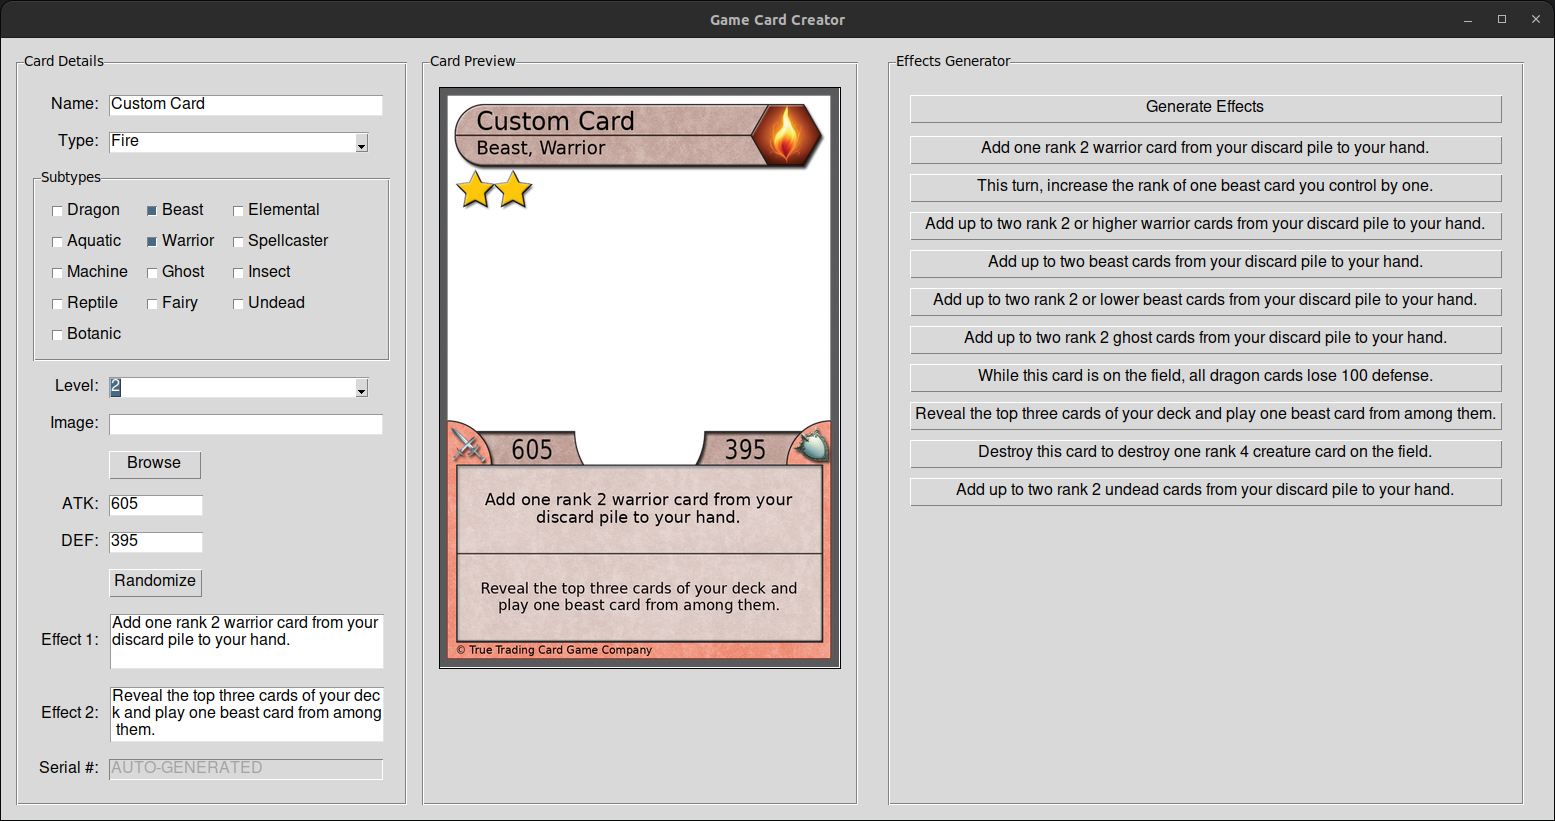
\includegraphics[width=\textwidth]{images/ui_sample.png}
	\caption{Screenshot of the \texttt{card\_maker\_ui.py} interface, showcasing a card preview with ``Nature'' type, level 4, and randomized ATK/DEF values.}
	\label{fig:card_maker_ui_screenshot}
\end{figure}

\subsection{Requirements}
\begin{itemize}
	\item Python 3.10+ with Tkinter (standard library) and \texttt{Pillow} (\texttt{pip install Pillow}).
	\item Companion scripts \texttt{create\_card.py} and \texttt{generate\_random\_effects.py} in the same directory.
	\item Effects CSV file (e.g., \texttt{effects/effects\_with\_placeholders.csv}) and PNG images in \texttt{../images/card pngs/}.
\end{itemize}

\subsection{Limitations}
\begin{itemize}
	\item Depends on external scripts and specific file paths, requiring proper project setup.
	\item No current implementation for saving card data to a spreadsheet (placeholder \texttt{print} only) at the time of writing this - the tool is still being developed.
	\item Effect generation may produce fewer than ten unique effects if the CSV pool is limited.
\end{itemize}